\documentclass[aspectratio=169]{beamer}
%
% Choose how your presentation looks.
%
% For more themes, color themes and font themes, see:
% http://deic.uab.es/~iblanes/beamer_gallery/index_by_theme.html
%
\mode<presentation>
{
    \usetheme{default}      % or try Darmstadt, Madrid, Warsaw, ...
    \usecolortheme{default} % or try albatross, beaver, crane, ...
    \usefonttheme{default}  % or try serif, structurebold, ...
    \setbeamertemplate{navigation symbols}{}
    \setbeamertemplate{caption}[numbered]
} 

\usepackage[english]{babel}
\usepackage[utf8x]{inputenc}
\usepackage{graphicx}
\usepackage{threeparttable}
\usepackage{eurosym}

\newenvironment{wideitemize}{\itemize\addtolength{\itemsep}{10pt}}{\enditemize}
\newenvironment{transitionframe}{
    \setbeamercolor{background canvas}{bg=white}
    \begin{frame}}{
    \end{frame}
}

\title[Your Short Title]{Knowledge is (less) power: experimental evidence from residential energy use}
\author{Katrina Jessoe \and David Rapson}
%\institute{}
\date{}

\begin{document}

\begin{frame}
    \titlepage
\end{frame}

\section{Summary}
\begin{frame}{Summary}
    \begin{wideitemize}
        \item RCT: effect of high-frequency information of electricity usage on price elasticity
        \item Informed households more elastic
        \item Evidence of learning and habit formation
    \end{wideitemize}
\end{frame}


\section{Background}
\begin{frame}{Background}
    \begin{wideitemize}
        \item Household electricity demand is inelastic
        \item Either inherently inelastic, or lack full information
        \item Infrequent billing: quantity used and usage by appliances unknown
    \end{wideitemize}
\end{frame}

\section{Experimental setup}
\begin{frame}{Experimental setup}
    \begin{wideitemize}
        \item Field experiment in Connecticut with United Illuminating Company, July and August 2011
        \item Sample of 437 households
        \item Random assignment into 3 groups
            \begin{wideitemize}
                \item Control: 207
                \item Price-only: 130
                \item Price+IHD: 100
            \end{wideitemize}
    \end{wideitemize}
\end{frame}

\begin{frame}{Pricing events}
    \begin{wideitemize}
        \item Day ahead (DA): Notified one day prior, 250\% increase
        \item 30 minutes (TM): Notified 30 minutes prior, 625\% increase
    \end{wideitemize}
    \center
    \resizebox{1\linewidth}{!}{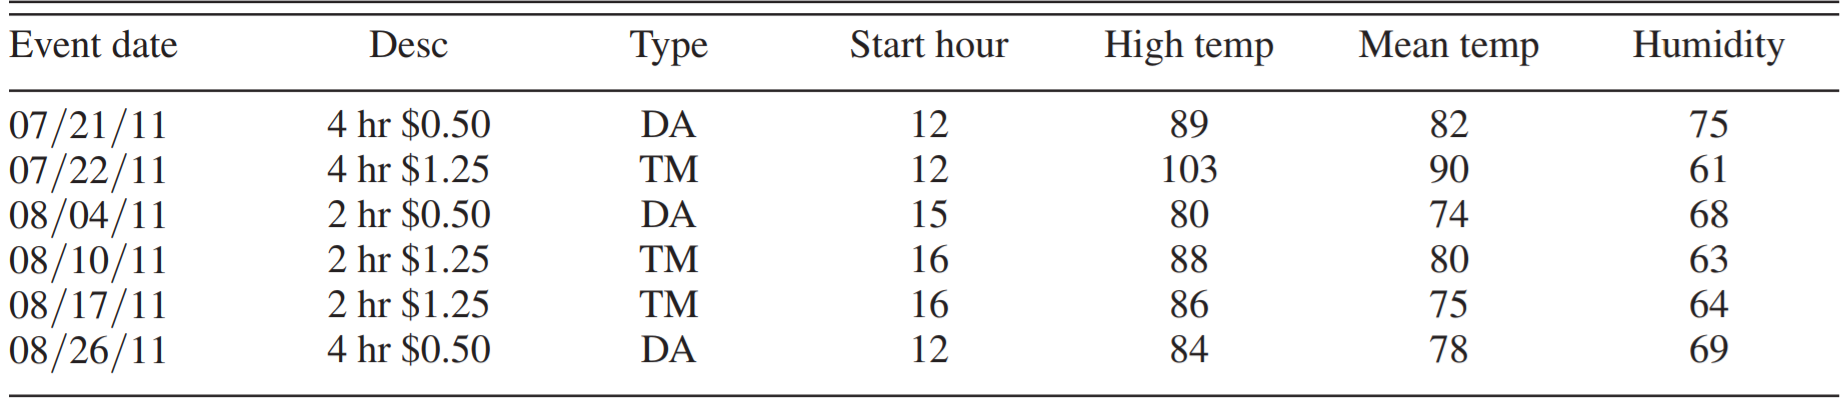
\includegraphics{pricing_events.png}}
\end{frame}

\begin{frame}{In-home display}
    \resizebox{0.45\linewidth}{!}{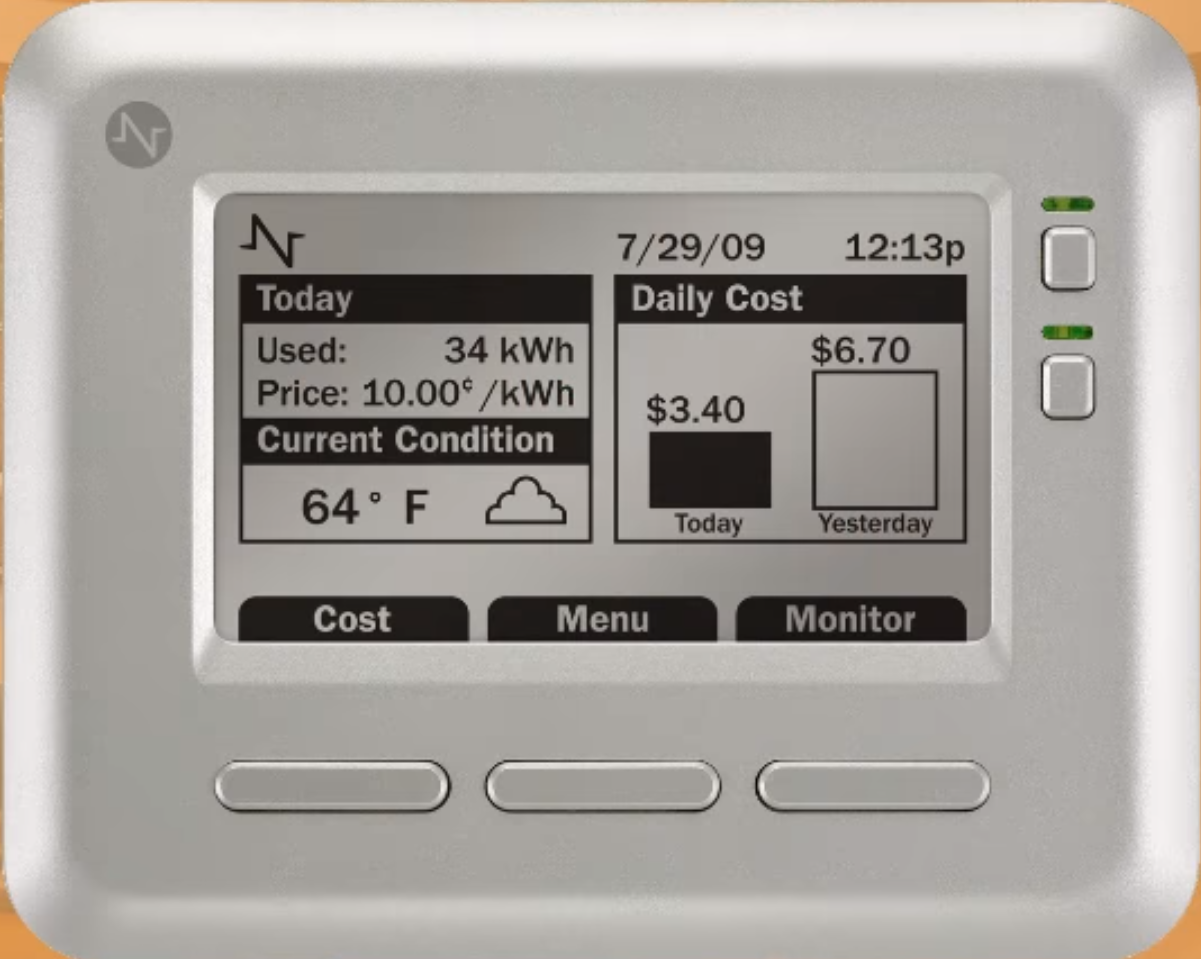
\includegraphics{ihd1.png}}
    \resizebox{0.45\linewidth}{!}{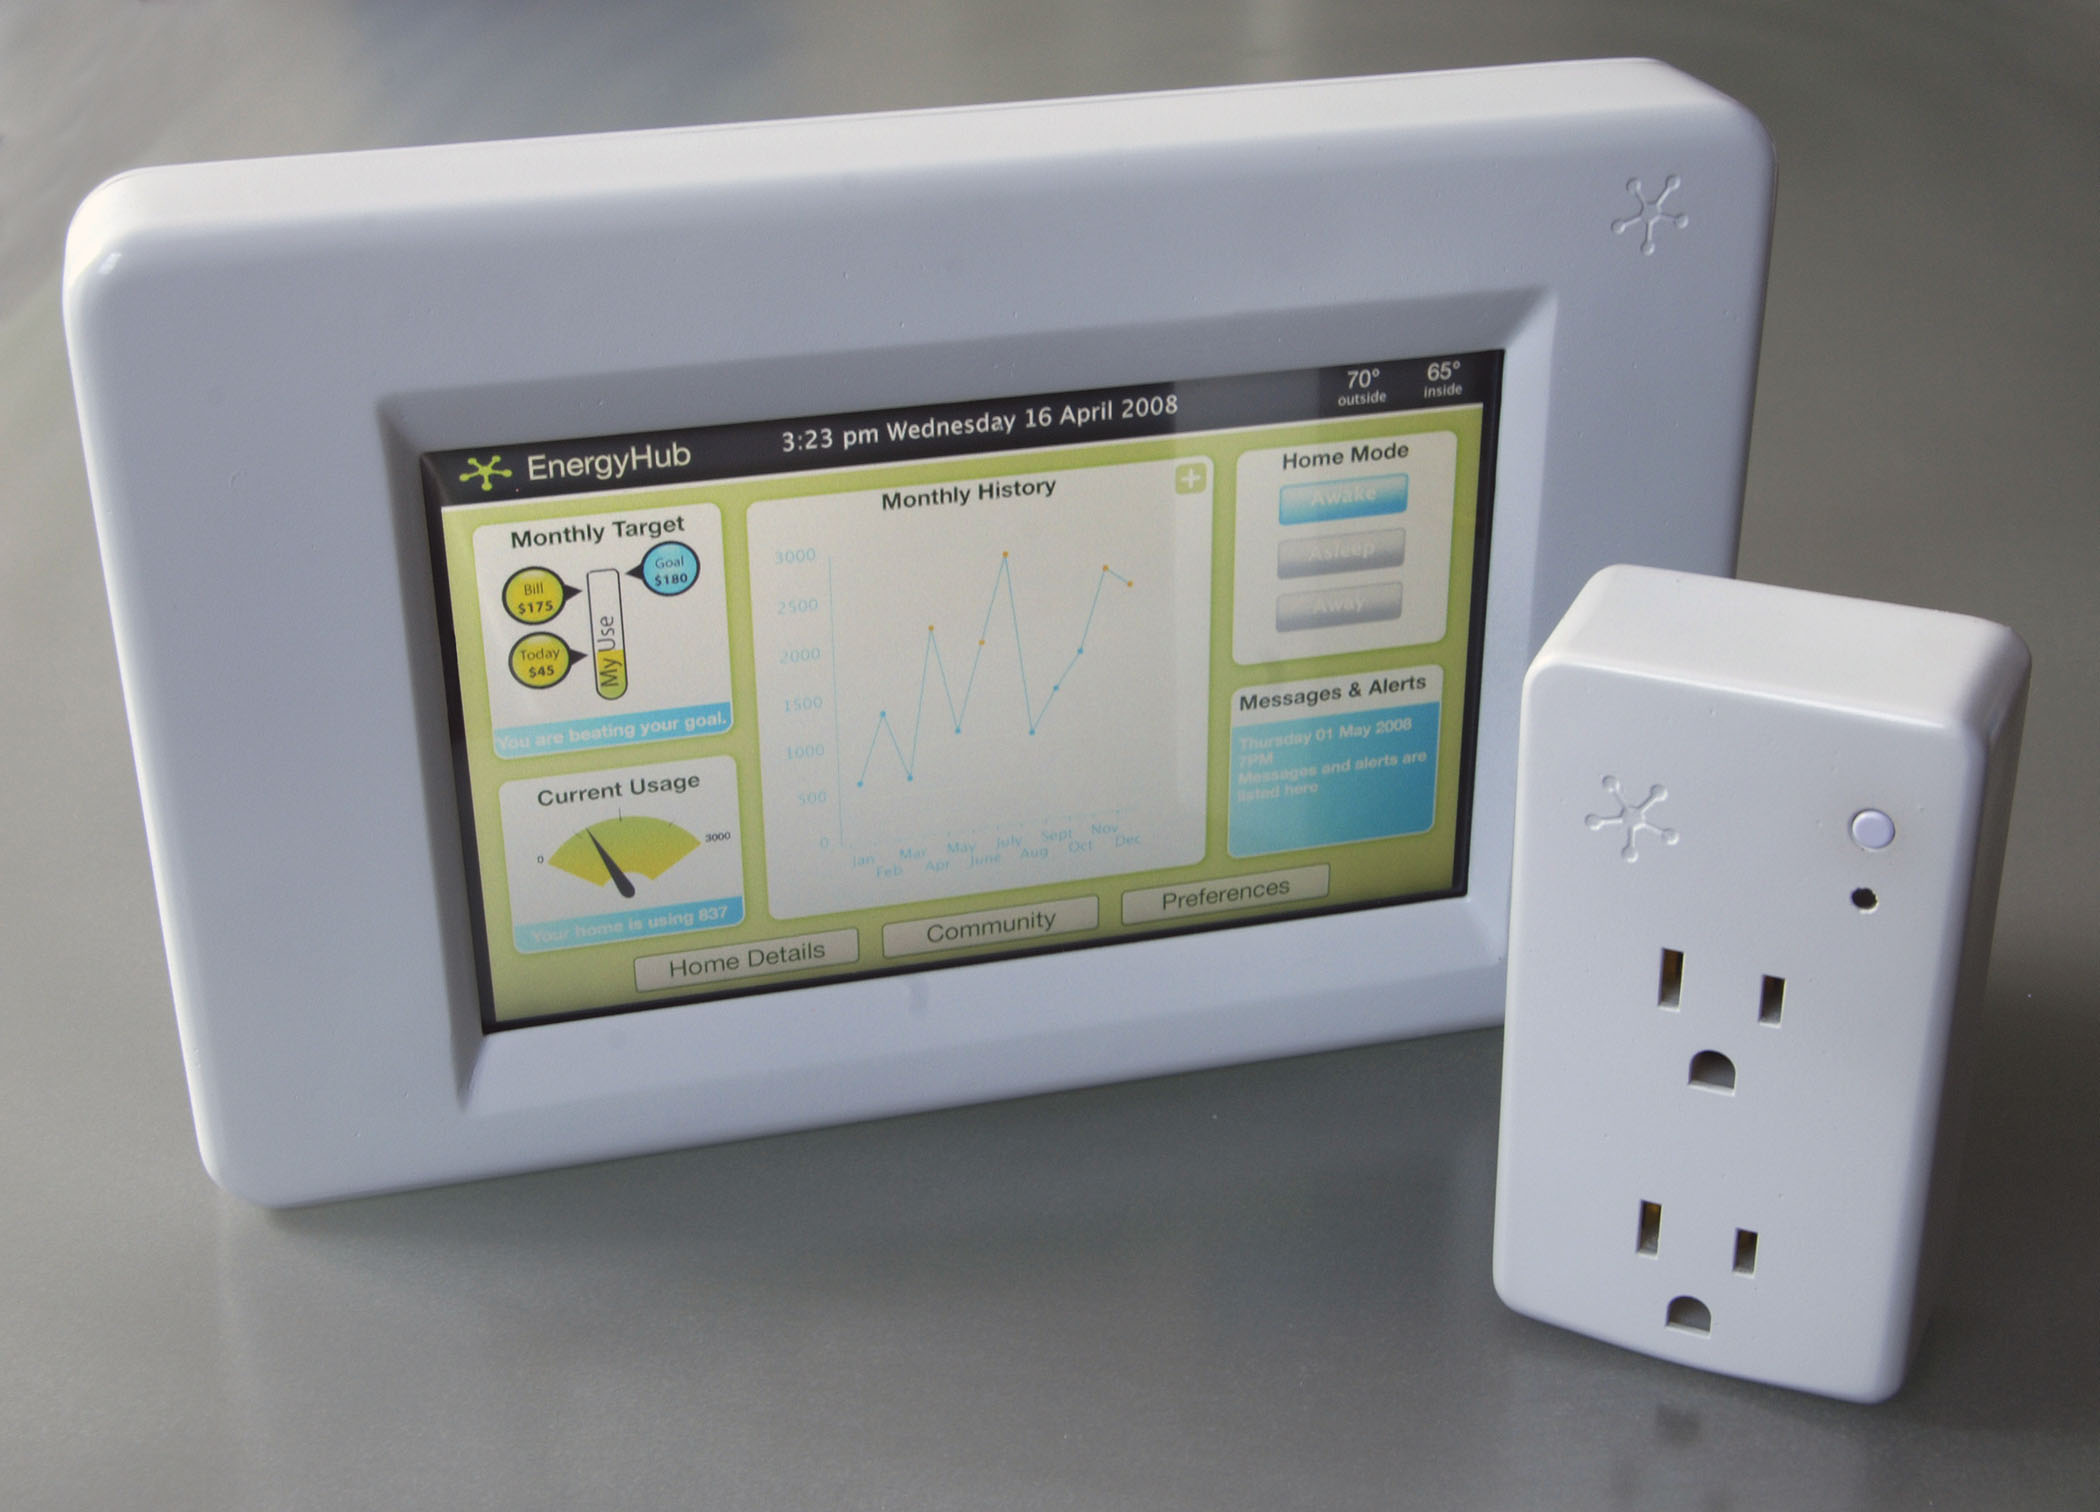
\includegraphics{ihd2.jpg}}
    Provides real-time usage, electricity price, estimated monthly usage and bill-to-date
\end{frame}

\begin{frame}{Data}
    \begin{wideitemize}
        \item High frequency meter data, 15-minute intervals
        \item Data on receipt of event notification
        \item 2 surveys: demographics, characteristics, frequency of use of IHD
        \item Software issues caused random missing observations
    \end{wideitemize}
\end{frame}

\begin{frame}{Balance}
    \center
    \resizebox{0.55\linewidth}{!}{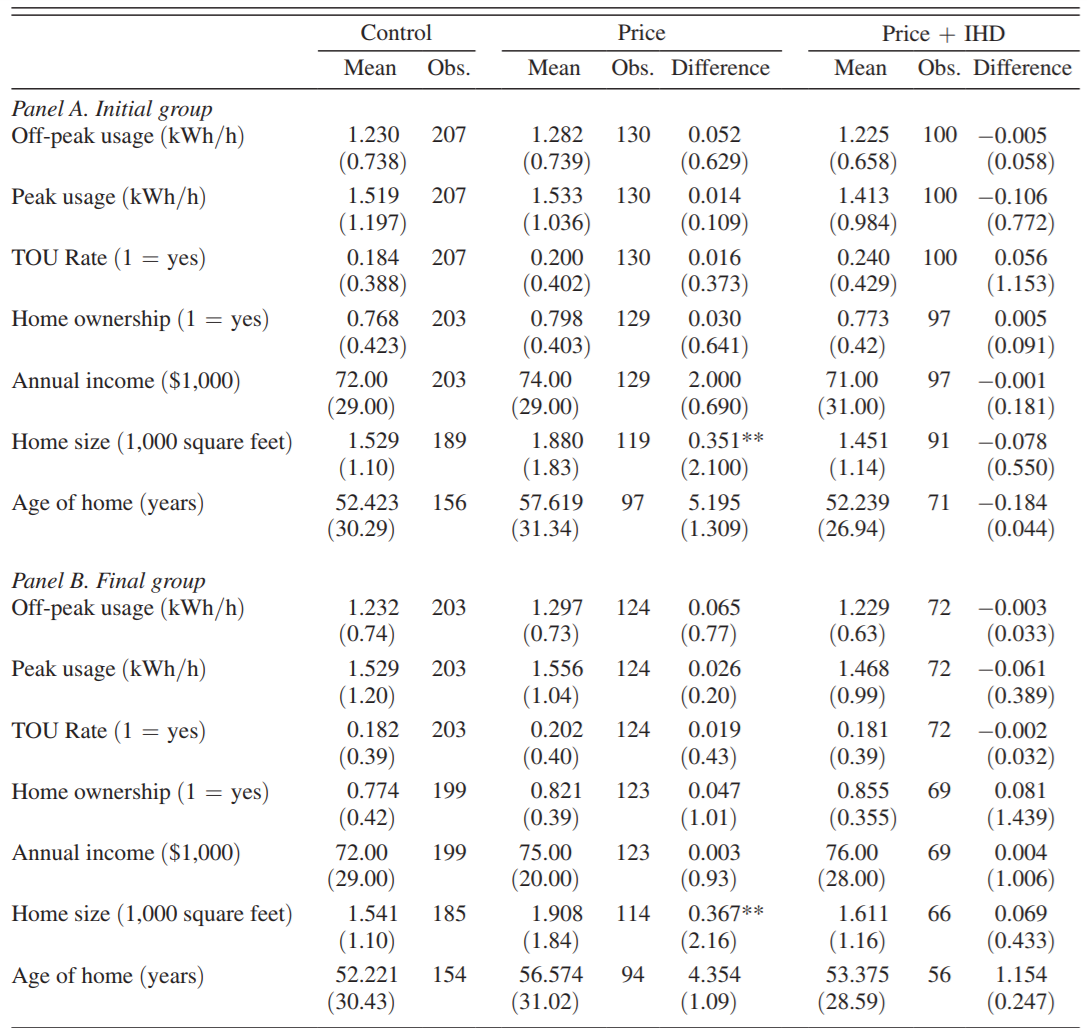
\includegraphics{balance.png}}
\end{frame}

\begin{frame}{LPM}
    \begin{wideitemize}
        \item Estimate LPM of treatment on mean off-peak usage and rate class; neither variable significant
        \item Estimate LPM of compliance on mean off-peak usage and rate class; rate class is significant
        \item Possible selective attrition
    \end{wideitemize}
\end{frame}

\begin{frame}{LPM results}
    \center
    \resizebox{1\linewidth}{!}{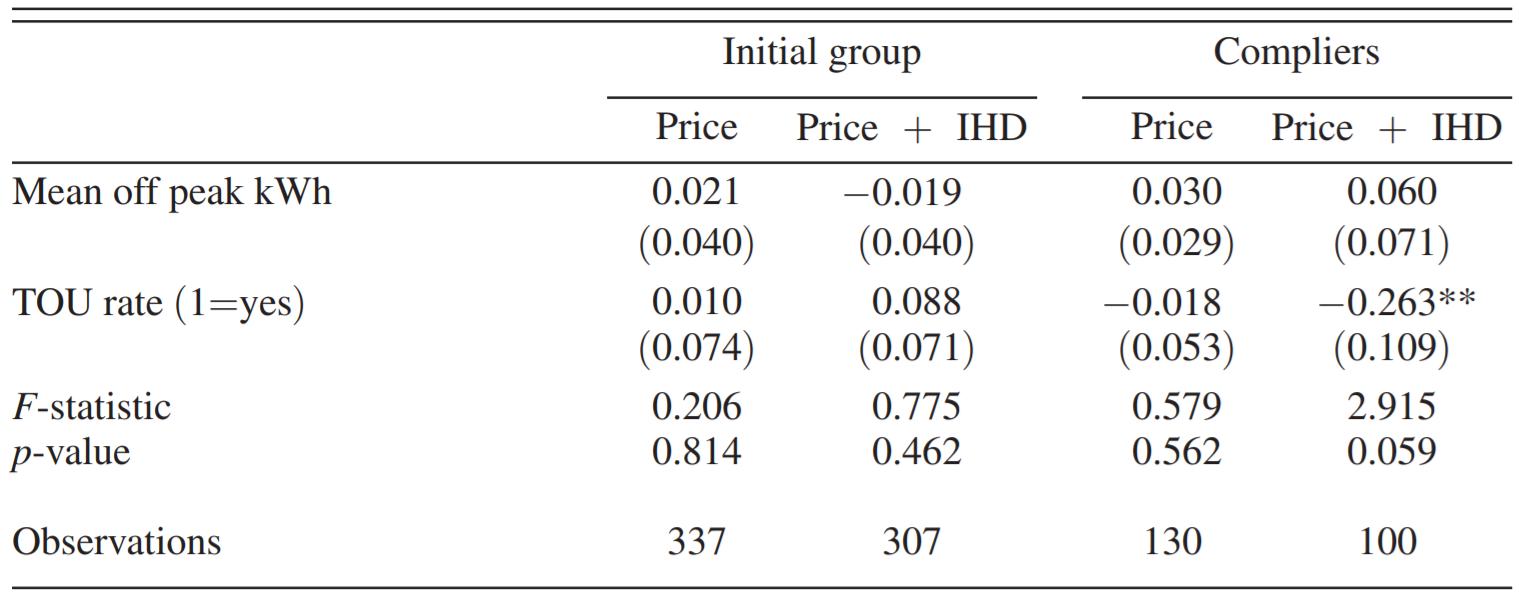
\includegraphics{lpm.png}}
\end{frame}

\section{Results}
\begin{frame}{Raw data 1}
    \center
    \resizebox{1\linewidth}{!}{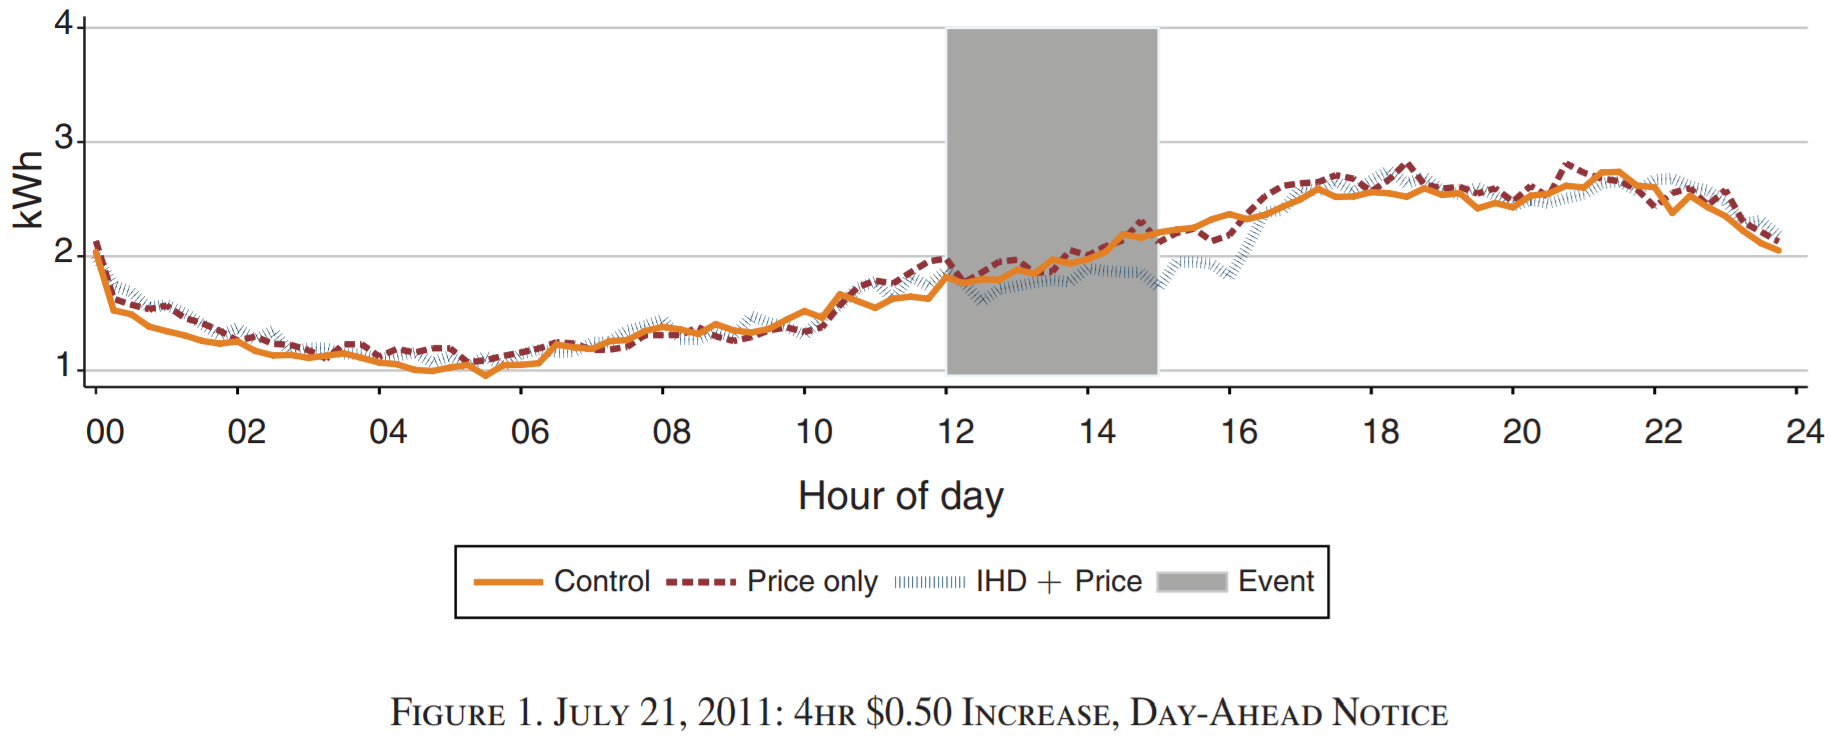
\includegraphics{raw1.png}}
\end{frame}

\begin{frame}{Raw data 2}
    \center
    \resizebox{1\linewidth}{!}{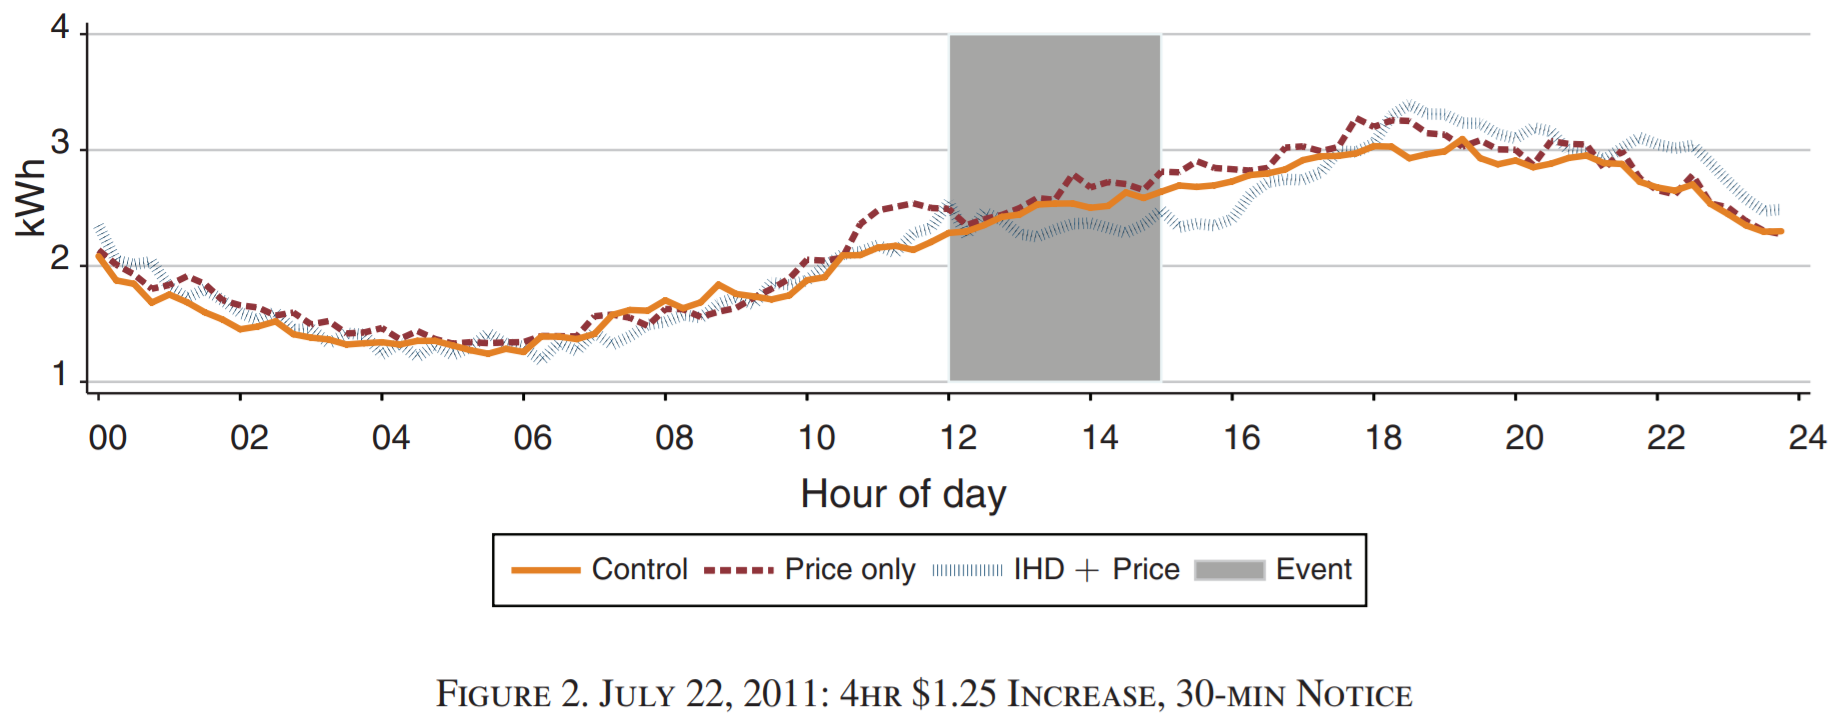
\includegraphics{raw2.png}}
\end{frame}

\begin{frame}{Raw data 3}
    \center
    \resizebox{1\linewidth}{!}{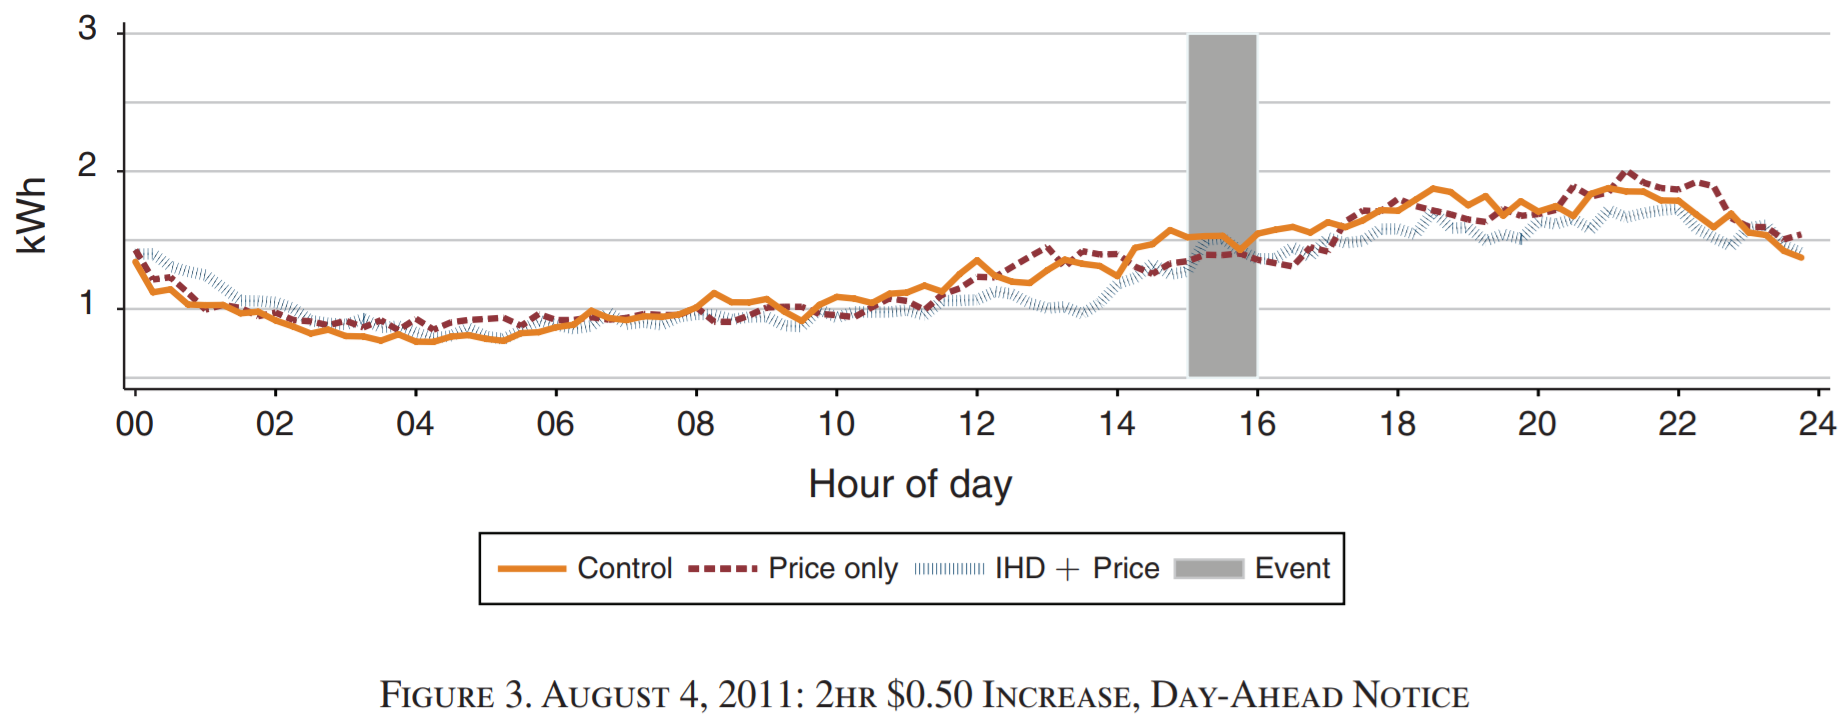
\includegraphics{raw3.png}}
\end{frame}

\begin{frame}{Raw data 4}
    \center
    \resizebox{1\linewidth}{!}{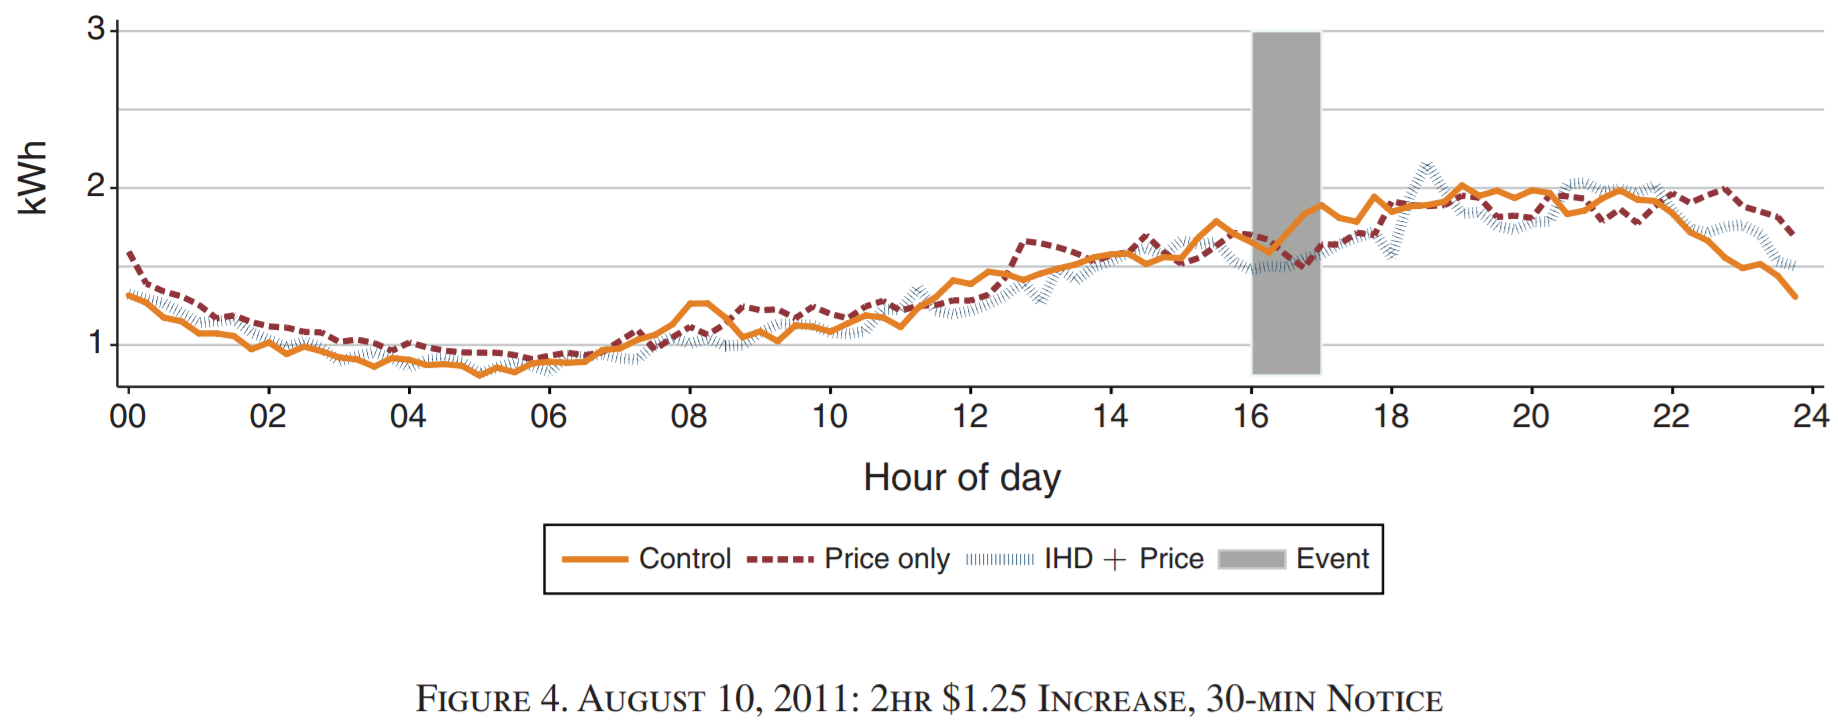
\includegraphics{raw4.png}}
\end{frame}

\begin{frame}{Raw data 5}
    \center
    \resizebox{1\linewidth}{!}{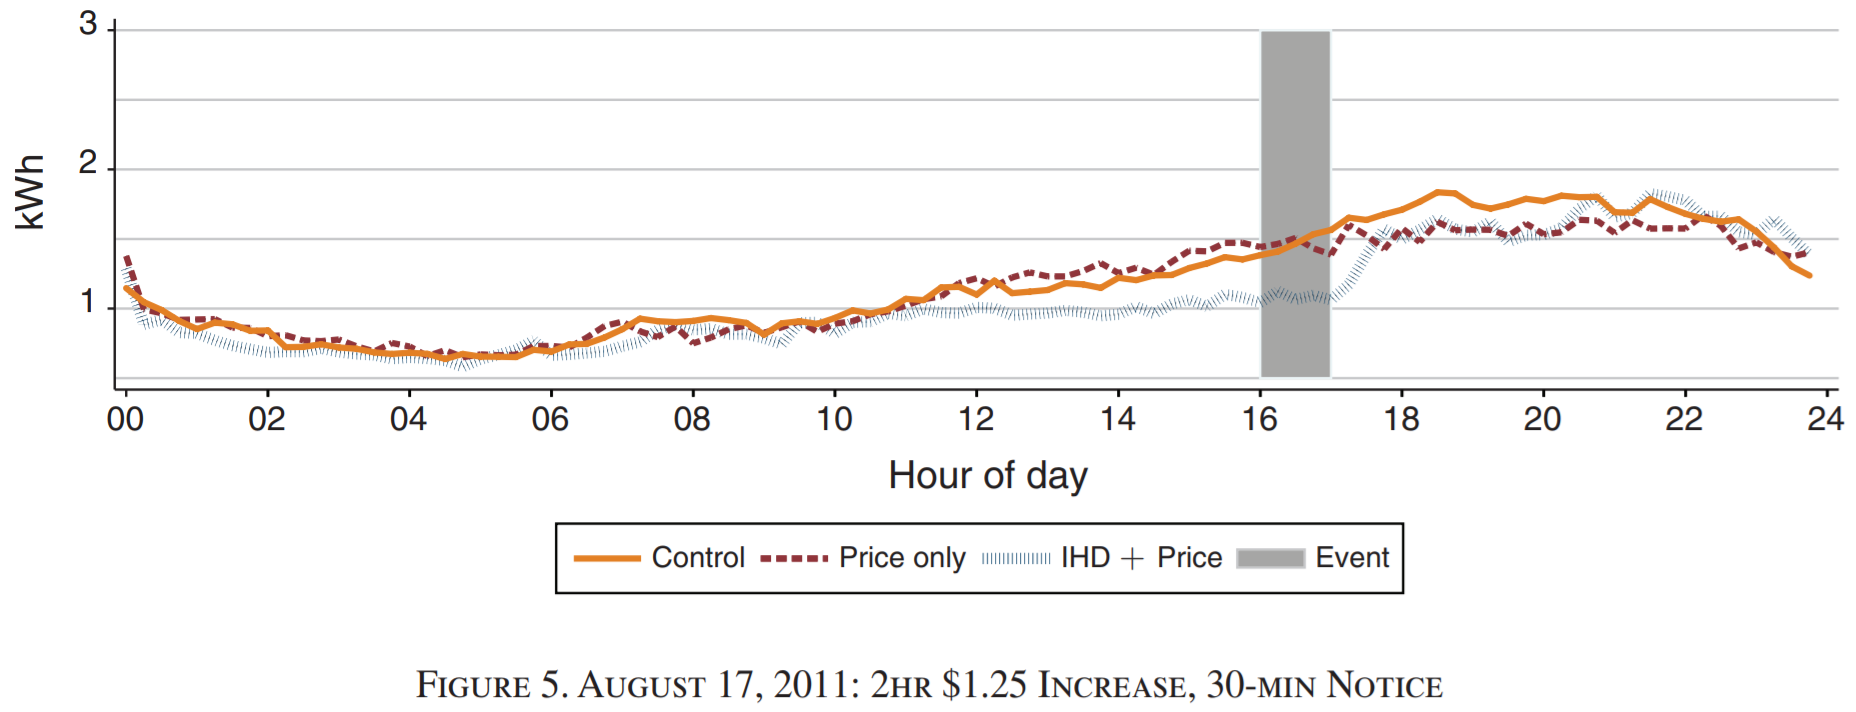
\includegraphics{raw5.png}}
\end{frame}

\begin{frame}{Raw data 6}
    \center
    \resizebox{1\linewidth}{!}{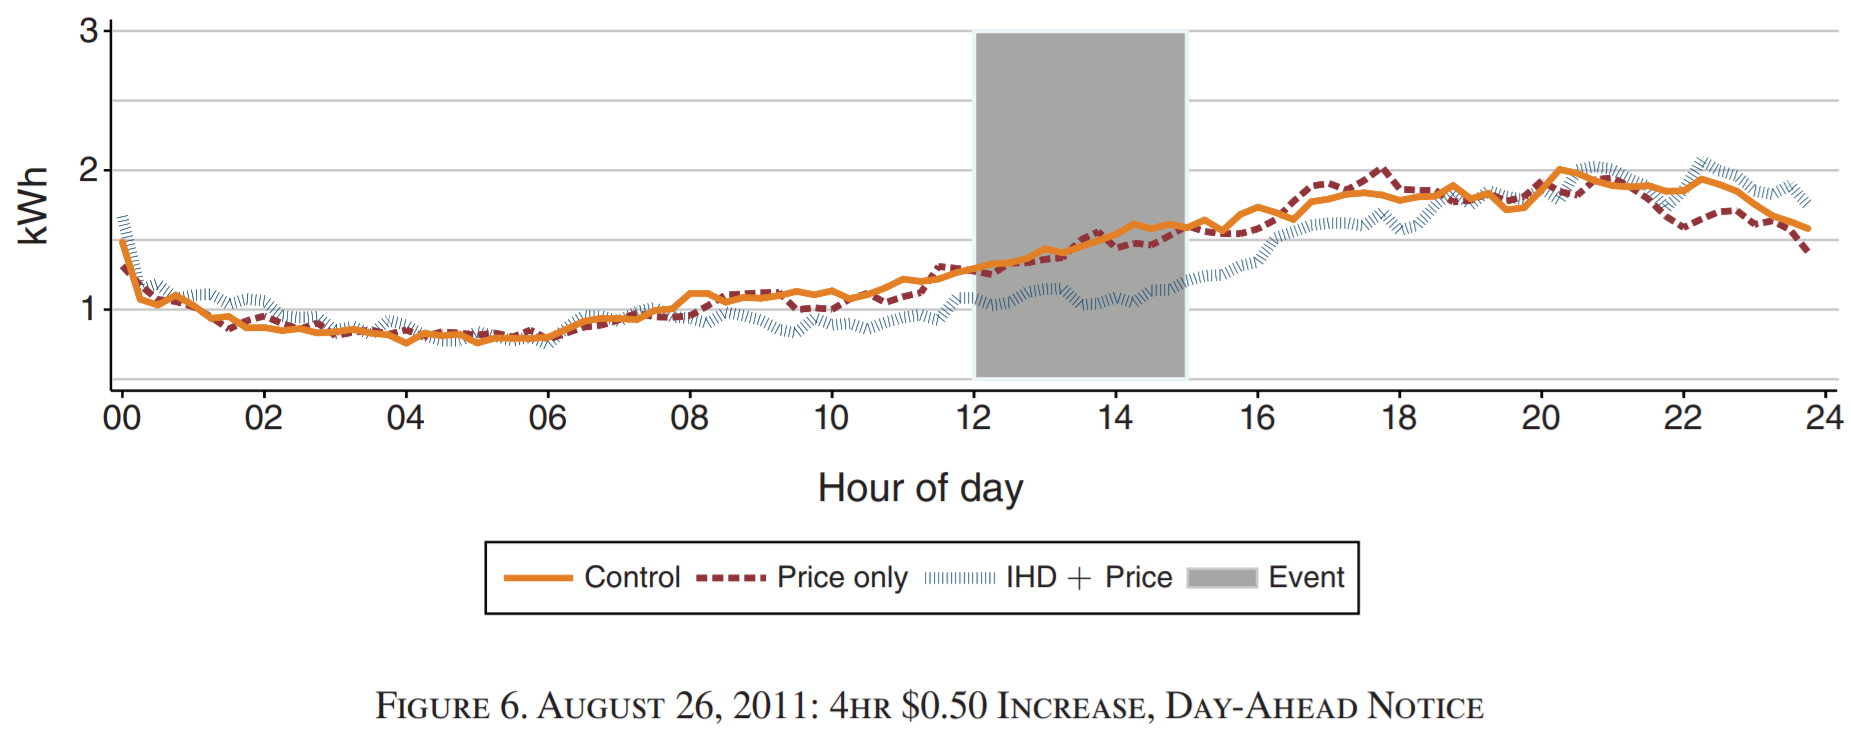
\includegraphics{raw6.png}}
\end{frame}

\begin{frame}{Difference in means}
    \center
    \resizebox{0.8\linewidth}{!}{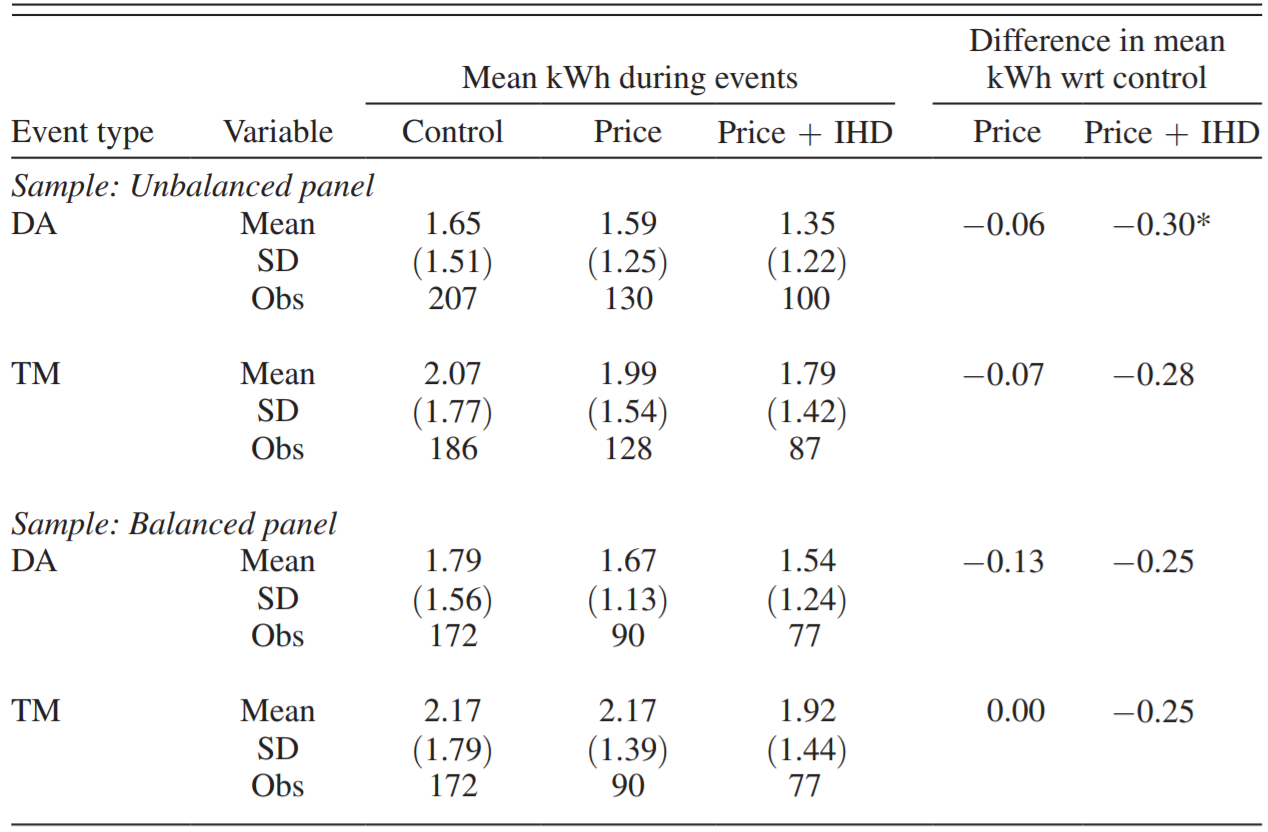
\includegraphics{diff_mean.png}}
\end{frame}

\begin{frame}{DiD estimation}
    \begin{wideitemize}
        \item Estimation equation:
            \begin{align*}
                q _ { i t } = \sum _ { g \in \{ P , P + I \} } \beta _ { g } D _ { i t } ^ { g } + \gamma _ { g } + \delta _ { e } + \mu _ { i t }
            \end{align*}
        \item Intent-to-treat (ITT) and Treatment-on-the-Treated (ToT) estimator
\end{wideitemize}
\end{frame}

\begin{frame}{DiD results}
    \center
    \resizebox{0.8\linewidth}{!}{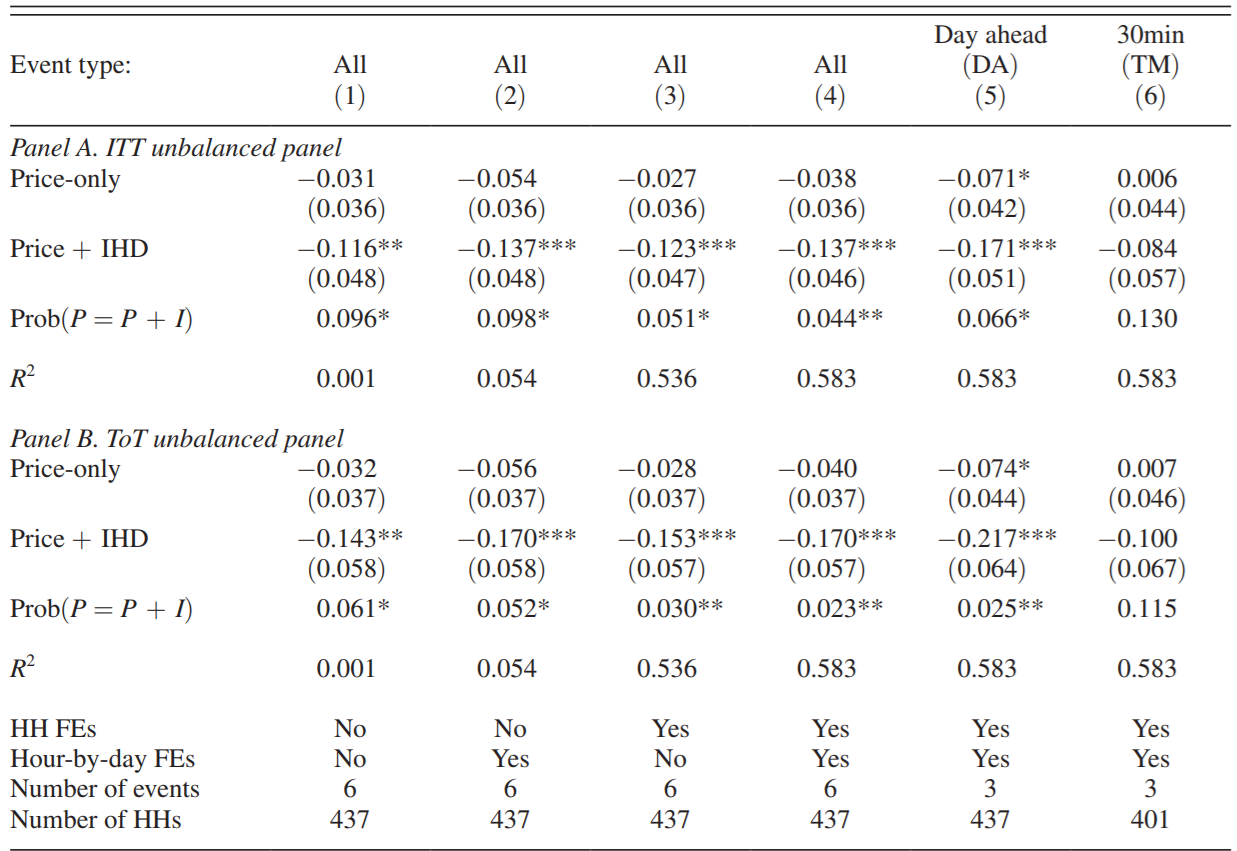
\includegraphics{results.png}}
\end{frame}

\begin{frame}{IHD effect?}
    \begin{wideitemize}
        \item 2 possible channels:
        \begin{wideitemize}
            \item increased awareness of price events
            \item learning
        \end{wideitemize}
        \item Rule out first channel
        \item Confirmation of receipt of notification indicates awareness of price events
    \end{wideitemize}
\end{frame}

\begin{frame}{Ruling out price salience}
    \begin{wideitemize}
        \item Interact treatment dummy with confirmation dummy:
        \begin{align*}
            q _ { i t } = \sum _ { g \in \{ P , P + I \} } \sum_{A \in \{ 0,1 \}} \beta _ { g } D _ { i t } ^ { g } \times 1 A _ { i t = A }  + \gamma _ { i } + \sigma _ { h } + \mu _ { i t }
        \end{align*}
        \item Idea: Conditional on confirmation, there is a difference in response
        \item Conditional on non-confirmation, no difference in response
    \end{wideitemize}
\end{frame}

\begin{frame}{Price salience results}
    \center
    \resizebox{1\linewidth}{!}{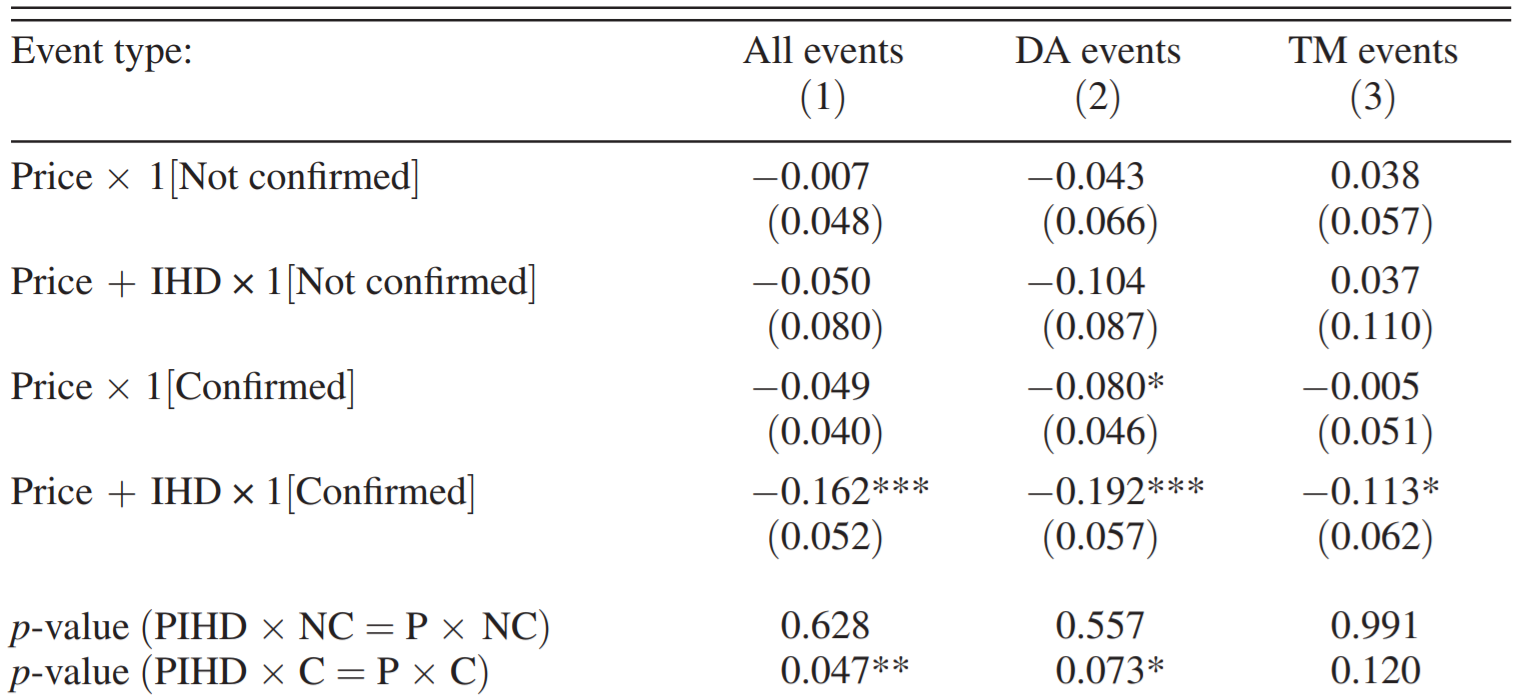
\includegraphics{confirmation.png}}
\end{frame}

\begin{frame}{Learning via IHD interaction}
    \begin{wideitemize}
        \item Frequency of interaction with IHD indicates learning
        \item Interact treatment dummy with interaction intensity
        \begin{align*}
            q _ { i t } = \sum _ { g \in \{ P , P + I \} } \sum_{A} \beta _ { g } D _ { i t } ^ { g } \times 1 A _ { i t = A }  + \gamma _ { i } + \sigma _ { h } + \mu _ { i t }
        \end{align*}
    \end{wideitemize}
\end{frame}

\begin{frame}{IHD interaction results}
    \center
    \resizebox{1\linewidth}{!}{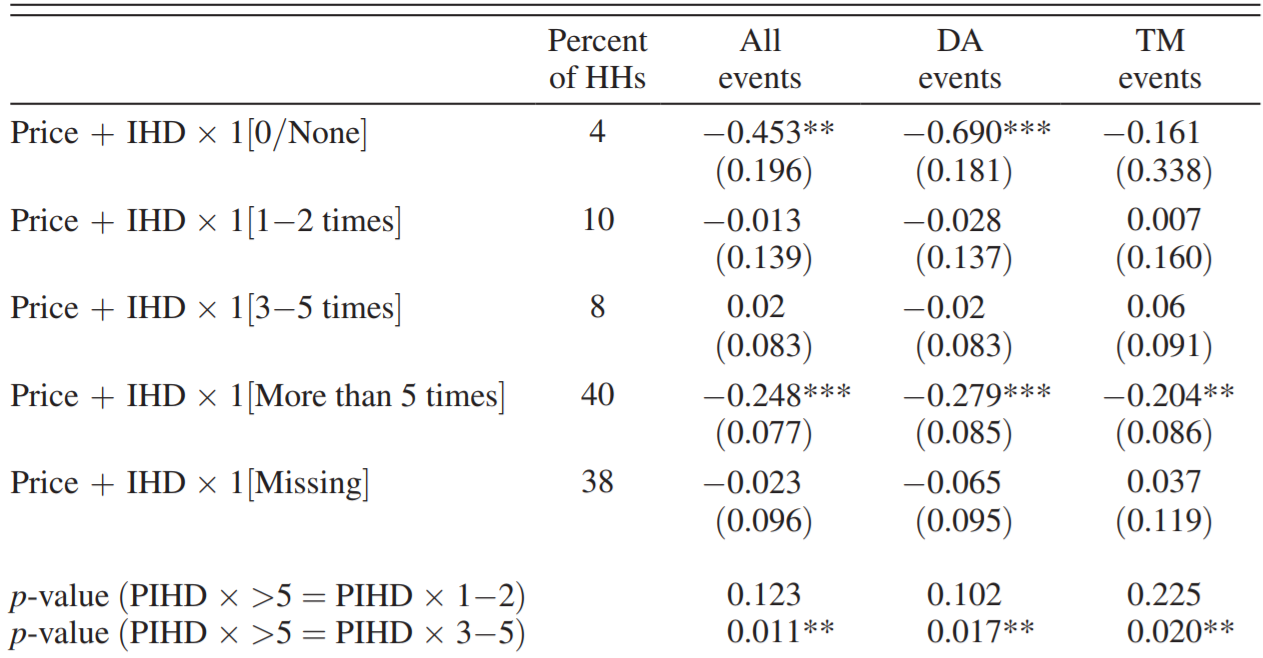
\includegraphics{ihd_freq.png}}
\end{frame}

\begin{frame}{Load-shifting and spillovers}
    \begin{wideitemize}
        \item Conservation during event may be offset by load-shifting
        \item Reduction in usage before and after event
        \item Add 2-hour before and after event indicators to ITT specification
    \end{wideitemize}
\end{frame}

\begin{frame}{Load-shifting and spillovers results}
    \center
    \resizebox{1\linewidth}{!}{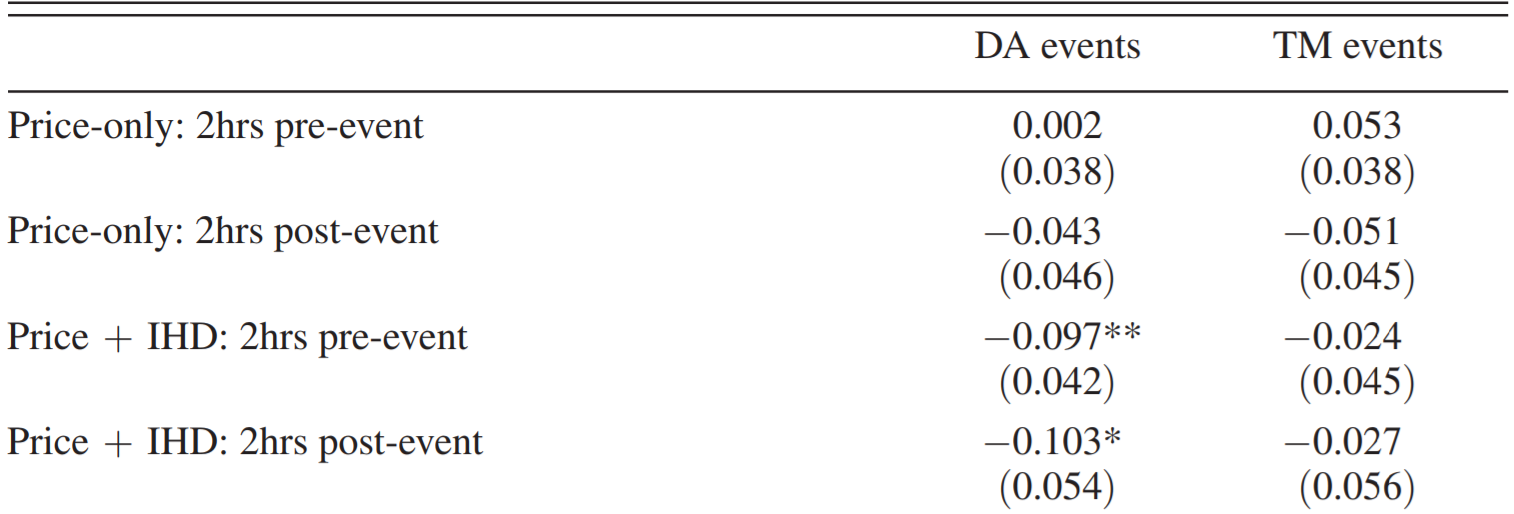
\includegraphics{prepost.png}}
\end{frame}

\begin{frame}{Habit formation}
    \begin{wideitemize}
        \item Multiple exposures cause reduction in usage outside of price events
        \item Estimate average daily decrease in usage at different hours of the day
        \begin{align*}
            q _ { i t } = \sum _ { g } \beta _ { g } D _ { i t } ^ { g } + \sum _ { g } \sum _ { h o d } \lambda _ { g , h o d } \times D _ { i } ^ { g } \times d + \gamma _ { i } + \sigma _ { h } + \mu _ { i t }
        \end{align*}
        \item $hod$ is hour-of-day binary indicator
        \item $d$ is running variable for day, 1 to 62
    \end{wideitemize}
\end{frame}

\begin{frame}{Habit formation results}
    \center
    \resizebox{0.85\linewidth}{!}{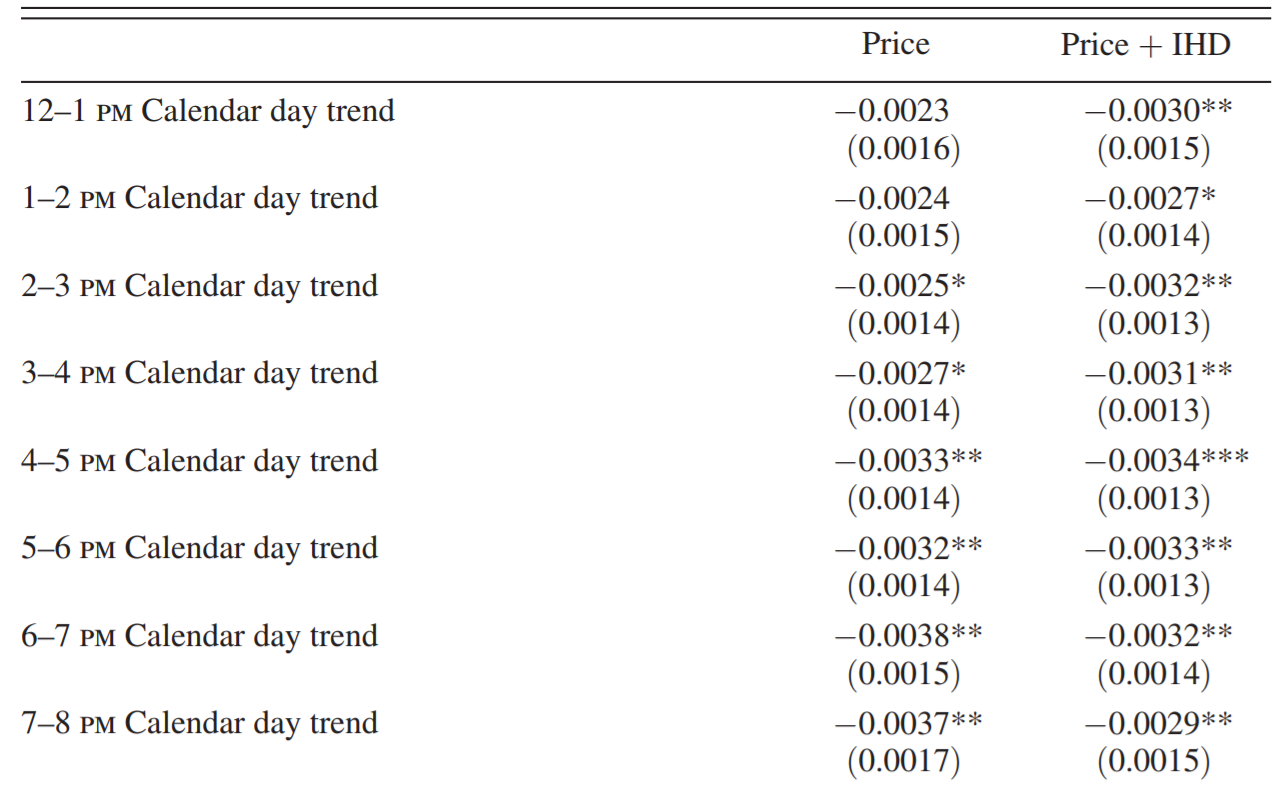
\includegraphics{habit.png}}
\end{frame}

\begin{frame}{Interpretation}
    \begin{wideitemize}
        \item Attenuation of main effect estimate due to reduction in baseline usage
        \item Larger spillovers for price+IHD indicates even larger effect of information feedback on elasticity
        \item Similar cumulative response irrespective of information feedback, but information may allow better response to short-run incentives
        \item Habit formation in both groups, possible large GHG abatement benefits
    \end{wideitemize}
\end{frame}
\end{document}
